\documentclass[letterpaper, 12pt]{article}
%%\documentclass[letterpaper, 11pt, twocolumn]{article}
\usepackage{url}
\usepackage{ctable}
\usepackage{overcite}
\usepackage{amsmath,amssymb}      % for \AA etc
\usepackage[onehalfspacing]{setspace}
\usepackage{graphicx}
\usepackage{fullpage, times}
\usepackage{algorithmic}
\usepackage{algorithm}
\usepackage{longtable}

\DeclareGraphicsExtensions{.pdf,.png}
\onehalfspacing

\bibliographystyle{jcics}

\usepackage{anysize}
%\marginsize{1in}{2in}{1in}{1in}
%\marginparwidth 1.75in
%\newcommand{\mnote}[1]{\marginpar{\raggedright{\footnotesize\textbf{#1}}}}

\def\imagetop#1{\vtop{\null\hbox{#1}}}

%%%
%%% Don't change the size of the figures as they are defined for
%%% a single column environment, which is what we will be submitting
%%% as
%%%

\begin{document}
\title{A Survey of Quantitative Descriptions of Molecular Structure}
\author{Rajarshi Guha${}^{\dagger}$ and Egon Willighagen${}^{\ddagger}$\\
${}^{\dagger}$NIH Center for Advancing Translational Science\\9800 Medical
Center Drive  Rockville, MD 20850 \\U.S.A.\\
${}^{\ddagger}$ Department of Bioinformatics - BiGCaT\\Maastricht University\\P.O. Box 616\\NL-6200 MD Maastricht\\The Netherlands
}
\date{}

\maketitle
\begin{abstract}
  Numerical characterization of molecular structure is a first step in
  many computational analysis of chemical structure data. These numerical
  representations, termed descriptors, come in many forms, ranging
  from simple atom counts and invariants of the molecular graph to
  distribution of properties, such as charge, across a molecular
  surface. In this article we first present a broad categorization of
  descriptors and then describe applications and toolkits that can be
  employed to evaluate them. We highlight a number of issues
  surrounding molecular descriptor calculations such as versioning and
  reproducibility and describe how some toolkits have attempted to
  address these problems.
\end{abstract}

\section{Introduction}

Computational methods play an important role in many chemical
disciplines ranging from drug discovery to materials science.
There are a plethora of techniques that differ in terms of
computational complexity, time requirements and so on. However the
common requirement underlying all these methods is a formal
description of a the molecular structure. There are many
ways to ``describe'' a molecule. A common approach is to describe the
connectivity, taking into account the types of atoms and bonds. In
other words, explicit representations of chemical structure such as
SMILES, MDL/Symyx SD files and so on. While these descriptions are vital to
modern chemical information systems, they do not necessarily allow
computational techniques to be directly applied to them.

Methods that aim to predict chemical and biological properties
generally require a numerical description of chemical structures. Such
numerical forms range from a set of 3D coordinates (which coupled with
appropriate atom types, is sufficient for methods such as quantum
mechanical (QM) approaches and docking to more abstract numerical
descriptions derived from 2D or 3D representations which can be useful
in statistical approaches. It is now possible to evaluate thousands of
numerical descriptors of chemical structure. As will be discussed
later, many of these descriptors are closely related or capture the
same information, allowing one to be substituted for another. The
choice of descriptors is a well-known problem and given a large
collection of them, approaches to identify a suitable subset have been
discussed extensively in the
literature~\cite{Miller:2002aa,Kohavi:1997gf}.

In addition to there being many possible descriptors defined in the
literature, there are also multiple implementations of a give
descriptor. These implementations are available in the form of
libraries (which require one to write a program to use them) or
complete applications (graphical user interface (GUI) or command
line). As a result, not only must one choose one or more descriptors
that are relevant to the problem at hand, but one must be concerned
about how they are calculated and whether such a calculation can be
reproduced across different implementations of those descriptors. It
is easy to understand \emph{why} two implementations of the same
descriptor can lead to different results - the primary reasons being
that the chemistry model that underlies the framework or toolkit used
to implement the descriptor is different. For example, a descriptor
that calculates the number of aromatic atoms may be implemented using
two toolkits with differing aromaticity models, and hence it is
possible that the values generated by the two implementations will
differ. Other sources of differences include parameters that may be
involved in the descriptor calculation and reference data values (such
as atomic radii, electronegativity values) that are employed during
descriptor calculation. While most implementations will employ the
same data sources for standard concepts (e.g., atomic weights), slight
differences in these types of input data can lead to differences in
the final descriptor value~\cite{Guha:2006ac}. As a result, in most
cases, two implementations of a descriptor do not usually give the
exact same value, though they are usually quite similar. Explicitly
explaining the differences may or may not be possible (it is usually
more difficult in the cases of commercial implementations for which
source code is not available)~\cite{Spjuth2010}.

\section{A Categorization of Descriptors}
\label{sec:categ-descr}

We have noted that a molecular structure can be characterized using
many numerical descriptors. In this section we describe a
categorization of descriptors. Admittedly, the grouping is somewhat
arbitrary but serves as a useful guide. In addition, the
categorization also takes into account the nature of the chemical
structure being considered - some descriptors are only useful when
applied to small molecules, whereas other descriptors are defined
specifically for polymers or protein structures.  Broadly, one can
classify descriptors based on the nature of structural information
they require.

Constitutional descriptors only require atom and bond labels and
usually represent counts of different types of atoms or bonds. While
very simplistic they can play a useful role in a variety of
applications ranging from summaries of physicochemical properties to
predictive modeling \cite{Bender:2005aa}.

Topological descriptors take into account connectivity along with atom
and bond labels. They consider the molecule as a labeled graph and
characterize it using graph invariants. In addition to graph
invariants, topological descriptors based on information theory such
as entropy have also been defined\cite{Dehmer:2009uq}. An advantage of
these descriptors is that do not require any intensive pre-processing
steps such as 3D coordinate generation and conformational analysis. In
addition, many graph invariants can be rapidly computed for graphs
corresponding to small molecule structures (even though they may be
computationally intractable on much larger graphs). While this class
of descriptors have been used extensively in predictive modeling
applications
\cite{Garcia-Domenech:2008aa,Randic:2001ad,Besalu:2001aa}, a key
drawback is their lack of interpretability. The abstract nature of
many graph invariants and information theoretic descriptors, their use
in predictive models makes it difficult to explain the model in simple
physicochemical terms, though various attempts have been made at
interpretations \cite{Todeschini:1975dq,Stanton:2003aa}.

Geometric descriptors require a 3D conformation as input and therefore
the computations are not as fast as topological descriptors which do
not require the 3D coordinate generation step. Nearly all geometric
descriptors work on a single conformation and for cases where multiple
conformation must be considered, an averaging procedure is usually
employed. Examples of these descriptors include the gravitational
index \cite{Katritzky:1996ly} and moment of inertia descriptors.
Geometric descriptors encompass many aspects of a molecular
structure. For example, a number of them characterize the molecular
surface. The simplest such example is the surface area descriptor (and
the corresponding volume descriptor). A simple extension of such a
descriptor is to characterize distributions of a physicochemical
property over the molecular surface such as the Charged Partial
Surface Area descriptors \cite{Stanton:1990aa} that characterize the
partial charge distribution over the molecular surfce. Note that
surface descriptor calculations based on analytical
\cite{Connolly:1983aa} or tesselation algorithms
\cite{Eisenhaber:1995qf} can be slow and that parametrized methods
such as the Topological Polar Surface Area (TPSA) \cite{Ertl:2000aa}
and VSA descriptors \cite{Labute:2008aa} that are based on
precalculated surface area values derived from a list of functional
groups.

It is important to note that there is a difference between the
information a descriptor captures and how it is calculated. The above
categories are based on input requirements. This gives rise to
situations where the molecular volume property can be
described by geometrical descriptors, e.g. using an analytical
approaches ~\cite{Eisenhaber:1995qf}, and with approximate,
constitutional descriptors, such as the very fast algorithm use by the
VABC approach~\cite{Zhao:2003fk} which is based on group
contributions.  The latter descriptor has been implemented in the CDK
and correlates well with other approximations to the molecular volume
(Figure \ref{fig:molvol}).

Another important class of geometrical descriptors are those that
describe molecular shape. This property is a key factor in ligand-receptor interactions and is
an important approach to virtual screening. A variety of descriptors
have been devised to characterize molecular shape. The use of
overlapping atom centered Gaussians to represent molecular shape
\cite{Grant:1995aa} represents a significant computational advantage
over the traditional analytical approach of intersecting hard spheres,
supporting extremely rapid shape comparisons \cite{Grant:1999vn}. An
alternative approach described by Ritchie et al \cite{Ritchie:1999kx}
employed a spherical harmonic based representation of surfaces, that
in contrast to the Gaussian approach allows one to generate
characterizations of the surface and hence the shape at varying
resolutions. Another approach to multi-resolution shape
representations is the use of $\alpha$ shapes
\cite{Edelsbrunner:1994aa}, which represent a parametrization of the
convex hull derived from the molecular coordinates. This approach has
been employed to characterize shape and volume \cite{Wilson:2009ys}
though it is more computationally intensive than the methods mentioned
previously. In addition to functional representations of molecular
shape, a number of simpler formulations have been defined. For
example, the ``shape signature'' approach described by Zauhar et al
\cite{Zauhar:2003fk} is a novel application of a ray tracing method
that generates a description of the molecular shape. Ballester et al
\cite{Ballester:2007aa} described the Ultrafast Shape Recognition
(USR) approach that characterized molecular shape in terms of the
distribution of distances between the atoms and a set of pre-defined
points. This procedure characterizes the shape in the form of a 12-D
real valued fingerprint. As a result, the calculation procedure is
rapid and once calculated shape similarities can be evaluated rapidly
via a simple distance calculation. It should also be noted that shape
indices based on the molecular topology have also been described
\cite{Kier:1985aa}, which are very rapid to calculate (somewhat
analogous to the VSA descriptors) but do not directly represent the
molecular shape and instead infer it from topological connectivity.

The last category consists of QM descriptors. These
descriptors can also be applied to problems such as QSAR models
(though of course the time complexity of QM derived descriptors do not
make them amenable for large scale virtual screening
applications). These descriptors can be evaluated at various levels of
theory. For example, partial charges, HOMO and LUMO energies are
commonly evaluated using semi-empirical methods, while Eroglu and
T\"{u}rkmen \cite{Eroglu:2007uq} described DFT-derived descriptors
such as electronegativity, hardness and ionization potential (though
Puzyn et al question the need for such a high level of theory
\cite{Puzyn:2008fk}).

The descriptor categories listed here are not necessarily distinct,
many hybrid descriptors have been described that combine one or more
categories. For example, the charge indices described by Galvez et al
\cite{Galvez:1994aa} combine partial charge information and
topological connectivity. Similarly the CPSA descriptors combine
surface area and partial charge information. When considering hybrid
descriptors, it is useful to note the autocorrelation descriptors that
characterize the distribution of molecular properties across a
molecule in terms of an autocorrelation function. These descriptors
may be based on topological or geometric distances and can be combined
with arbitrary molecular properties \cite{Moreau:1980aa,Broto:1984aa}.

\subsection{Fingerprints}

Besides the numerical descriptors outlined so far, another useful
approach are those of fingerprints. Traditionally, fingerprint descriptors are
represented in the form of bit strings. These binary fingerprints can be
divided into hashed fingerprints, where substructures (such as paths
of length $n$) are converted to a string representation and then
hashed into a randomly selected bit positions, or keyed fingerprints,
where each bit position corresponds to a unique substructural
feature. The nature of the features can range from simple functional
groups (hydroxyl, carbonyl) and topological substructures (paths,
chains, cycles) to atom environments \cite{Bremser1978,Bender:2004aa}
and pharmacophoric elements \cite{Renner:2006aa}. Depending on the
definition, fingerprints can work with topology only or may require 3D
conformations. The latter class of fingerprints are usually related to
3D pharmacophores and most fingerprint definitions only require
connectivity information. 

Fingerprints are a compact representation of a chemical structure and
are used in a variety of ways ranging from database searches looking
for similar structures or substructures to virtual screenings studies
\cite{Sun:2006kx}. In many search applications, the binary nature of
fingerprints allow for efficient algorithms to compare molecules and
evaluate similarity and a number of heuristics have been developed
that allow for rapid similarity searches
\cite{Baldi:2008aa,Swamidass:2007ab}. In virtual screening scenarios,
fingerprints can be used as features. In many cases, the entire
fingerprint is employed as a set of independent variables. Since this
can lead to poor predictive models, some sort of feature selection is
usually employed and there have been studies that address the problem
of identifying subsets of bits from a fingerprint that lead to optimal
performance in predictive models (albeit, usually in a target-class
specific manner) \cite{Xue:2004fk}.

\subsection{Describing other chemistries}

We next consider descriptors that are designed for specific classes of
molecular systems.

\textbf{Descriptors for polymeric systems} These systems represent a
challenge for descriptor development. There have been reports that
employed traditional small-molecule descriptors
\cite{Mattioni:2002dq,Katritzky:1998cr} that consider the polymer in
terms of the individual monomers. A number of approaches have been
described that includes both deterministic, geometry derived
descriptors \cite{Edvinsson:2003bh} as well as stochastic methods
\cite{Gonzales-Diaz:2003ly}. For the case of polypeptides the
descriptors generally tend to be based on the individual amino
acids. Examples include the VHSE family of descriptors described by
Mei et al \cite{Mei:2005kx}, a set of side chain descriptors from
Collantes and Dunn \cite{Collantes:1995vn}, field based descriptors
\cite{Norinder:1991ys} and the AAindex database
\cite{Kawashima:1999zr} which allows rapid lookup of amino acid
properties.

\textbf{Descriptors for inorganic compounds} Inorganic materials are
sufficiently different from small molecules that traditional
descriptors are not very useful. Recently, a number of descriptors for
inorganic materials are very similar to constitutional descriptors -
essentially counts of various crystal parameters such as accessible
surface areas and volumes
\cite{Willems:2012zr,Haranczyk:2010ys,Mackay:1984ve}. Other
descriptors characterize the periodic voids of porous materials via
tesselation methods \cite{Anurova:2009ly,Carr:2009kx}.

Other methods developed for crystal structures have been developed
too, for example, using a radial distribution
functions~\cite{Willighagen2005}, which capture the packing of organic
crystal structures. Such approaches have been used to cluster crystal
structures~\cite{Wehrens2006} and compare
properties~\cite{Willighagen2007}.

\textbf{Bioactivity as a descriptor} While the descriptors mentioned
so far are derived from some form of chemical structure, an
alternative approach is to employ observed biological activities of a
molecule as descriptors of that molecule.  This approach was taken by
Sedykh et al \cite{Sedykh:2011fk} who hypothesized that dose response
data points from high throughput dose-response assays could be employed
as biological descriptors. They observed that when such descriptors
were combined with traditional chemical structure descriptors, the
predictive performance of models developed using the combined set was
better than those developed using conventional approaches. A similar
approach can be taken using the PASS methodology
\cite{Poroikov:2007aa}, though this is an indirect method - one must
predict the PASS profile from the chemical structure, which can then
be used in subsequent predictive models.

\textbf{Atom and bond descriptors} It should also be noted that various
toolkits also calculate descriptors for chemical entities like atoms and
bonds. These descriptors include simple element property descriptors,
but also geometrical descriptor, such as radial distribution functions
that describe the chemical environment of those atoms. These,
for example, have been used to predict proton shift in 
nuclear magnetic resonance~\cite{AiresDeSousa2002}. Similarly, bond
descriptors can be used to predict bond properties.

\section{What is a Useful Descriptor?}
\label{sec:what-usef-descr}

Given that we can generate thousands of descriptors,  it is critical to ask, what
makes a descriptor useful? Fundamentally, a descriptor must correlate
structural features with some physicochemical property and show
minimal correlation with other descriptors. In addition, a generally
useful descriptor will be applicable to a broad class of
molecules. Furthermore, a descriptor should show minimal
degeneracy. That is, the descriptor should generate different values
for structurally different molecules, even if the structural
differences are small. An example is the case of stereochemistry. Most
constitutional and topological descriptors that are not designed to take this into account will
generate the same numerical values for all the stereoisomers of a
given chiral molecule. We would consider such a descriptor to be
degenerate. In addition to degeneracy, a descriptor should be
continuous, in the sense, that small structural changes should lead to
small changes in the value of the descriptor.

The requirements listed here ensures that subsequent analyses
involving descriptors are robust. But in addition to numerical
robustness, it is important for many scenarios that the descriptor
have some form of physical interpretability.  For example, a model
that employs descriptors to predict cytoxicity will be most useful if
it is numerically accurate as well as providing insight into which
structural features confer toxicity. In such a scenario, abstract
descriptors do not allow us to provide a physical explanation of the
models predictions. Another scenario is the ability to map descriptor
values back to the structure for visualization purposes such as the
``Glowing Molecule'' depictions of Segall et al
\cite{Segall:2009fk}. Such visualizations are practical only when
descriptor values can be related to structural features. Examples
include surface based descriptors such as CPSA's as well as explicit
structural descriptors such as paths, chains etc.

However, there are certain scenarios where some of the above
characteristics are \emph{undesirable}. One such scenario is in the
safe exchange of structures, such that two parties can perform
analyses on the structure-derived data, without having to know the
structures explicitly. In such cases, the ability to go from a set of
descriptor values back to a chemical structure should be minimized. It
has not been conclusively proven that such a ``one-way'' descriptor
can be defined. For example Masek et al \cite{Masek:2008aa} have shown
that one can regenerate a target structure (or substructural features)
or a set of closely related analogs given a combination of descriptors
such as BCUTs. Tetko \textit{et al.} \cite{Tetko:2005fk} suggest an approach to
prevent reverse engineering but avoid the use of descriptors and
instead sharing structures of related molecules, rather than the
molecules of interest. One could also employ degenerate descriptors,
which would represent a large family of molecules, such that the
target molecule would be hidden. This is likely unreliable as it would
be difficult to perform analyses (e.g., predictive models) with such
descriptors.

\section{Descriptor Implementations}
\label{sec:descr-impl}

A variety of descriptor implementations are available, with most
cheminformatics toolkits providing implementations of a common set of
descriptors and fingerprints. Table~\ref{tab:impl} summarizes the
descriptor classes implemented by several toolkits and
applications. Note that due to space limitations this is not a
comprehensive list of implemented descriptors across different
applications and the reader is referred to the documentation
accompanying the software packages.

While library calls for descriptor evaluation is the most flexible
approach, it is not useful for non-programmers as well as users who
simply need a descriptor matrix for modeling or searching. As a
result, GUI or command line wrappers around descriptor APIs enable
easier usage. The CDKDescUI application
(\url{http://rguha.net/code/java/cdkdesc.html}) is a Java Swing
application that exposes the Chemistry Development Kit (CDK) descriptor and fingerprint API's. It
allows the users to specify a SMILES or SD file and evaluate a
selected set of descriptors or fingerprints and export them to a text
file. The application also has a command line mode that can be run in
server environments. A similar application is PaDEL \cite{Yap:2011fk}
that includes the CDK descriptors and also implements a number of
additional descriptors such as the extended topochemical atom
descriptors \cite{Roy:2004uq}, McGowan Volume \cite{Zhao:2003kx}, and
the Klekota \& Roth substructure counts \cite{Klekota:2008vn}.

There are also web interfaces wrapping descriptor calculation tools
and some of these interfaces have a programmable feature. For example,
AMBIT2 implement the OpenTox API providing a REST-like interface
to descriptor calculation~\cite{Jeliazkova2011,Hardy2010} (see Figure~\ref{fig:tools}). Another
online application programming interface for descriptor calculation
is provided by the SADI platform, which, like AMBIT2, uses semantic
web technologies for descriptor calculation~\cite{Chepelev2011b}.

In addition to libraries and their wrappers there are various GUI
applications that allow easy descriptor calculations. Examples include
Bioclipse \cite{Spjuth:2007aa} (see Figure~\ref{fig:tools}), MOE (Chemical Computing Group) and
Maestro (Schr\"{o}dinger, Inc.). Workflow tools are also a useful
class of applications for descriptor generation and allow one to
easily generate descriptors from multiple sources~\cite{Truszkowski2011} (see Figure~\ref{fig:tools}). Given the focus of
this article on Open Source implementations, we have noted the
availability in Table \ref{tab:impl}. While a number of
implementations are not strictly Open Source according to OSI
definitions, the fact that they provide free academic licenses does
allow them to be used somewhat freely.

Due to our experience with the CDK project we provide a brief overview
of the architecture of the descriptor calculations implemented by the
CDK. First, the toolkit explicitly differentiates between atom, bond
and whole molecule descriptors. There are a total of 30, 6 and 51
descriptor algorithms for atoms, bonds and molecules respectively. Note that
each individual descriptor algorithm may calculate multiple descriptors. For example,
the CPSA descriptor evaluates 30 individual descriptor values. Thus for a given
molecule it is possible to generate approximately 300 descriptor
values.

Every descriptor implements an interface allowing them to
return values in a uniform manner, viz., via a \texttt{DescriptorValue}
object (see Figure~\ref{fig:cdkapi}). This class can represents the result
of a descriptor calculation and includes both the descriptor values
(via a \texttt{IDescriptorResult} object) as well as meta-data on the
descriptor itself via a \texttt{DescriptorSpecification} object (see
below for more details). The descriptor classes are designed such that
in the event of a calculation error (invalid, missing or nonsensical
input), null values are returned, rather than throwing an
exception. This is useful during automated descriptor calculation,
where one desires a ``rectangular'' descriptor matrix, from which one
could filter out the undefined descriptors. While the user can pick
and choose specific descriptors to calculate, the API provides a class
(\texttt{DescriptorEngine}) to specifically evaluate all or a subset
of descriptors for a molecule at one go.  Currently the descriptor
implementations are not threadsafe, making them unsuitable for
parallelization. This is a drawback since many of the descriptors can
be slow. For example, the $\chi$ descriptors \cite{Kier:1976aa} are
implemented using SMARTS matching to identify the various paths and
chains described by Kier \textit{et al.}, rather than explicitly walking the
molecular graph.

\subsection{Comparing implementations}
\label{sec:comp-impl}


Given the multiple implementations of many descriptors, it is natural
to compare their performance. As noted previously, it is desirable,
but unlikely, that implementations of the same descriptor using
different cheminformatcs toolkits will be identical. Gupta et al
employed SMARTS based descriptors from the CDK and MOE to develop
decision tree models to predict human liver microsomal metabolic
stability \cite{Gupta:2010uq}. Their results indicated very similar
performance between the two implementations. In general, one would
expect a high degree of correlation between different implementations
of well-defined descriptors. Here ``well defined'' indicates that the
underlying parametrization or chemistry model is completely specified,
so that different implementations use them identically. For example,
correct implementations of the TPSA descriptor are expected to
correlate very well, and this is shown in Figure \ref{fig:tpsa} for
the ACD Labs and CDK implementations.

A number of physicochemical descriptors commonly employed in
predictive modeling are themselves models of an experimental
property. For example, log P can be experimentally measured and a
number of algorithms have been developed to predict $\log P$
\cite{Wang:1997aa,Wildman:1999aa}. Given the utility of log P in drug
discovery, a number of implementations are available. Given that this
descriptor is a surrogate for an actual experimental property, it is
reasonable to compare calculated log P values from different
implementations to the experimentally observed values, rather than
between themselves. Figure \ref{fig:logp} compares computed log P
values from the CDK (specifically, an implementation of the XlogP
method), ChemAxon and ACD Labs for a set of 10,000 molecules taken
from the logPstar dataset.

\subsection{Descriptor Naming \& Versioning}
\label{sec:descr-vers}

As noted above, different implementations of the same descriptor can
generate slightly different values depending on the underlying
chemistry model, differences in reference values and so on. Even
within the same software implementation, different versions of the
same descriptor can generate different values. Thus to maintain
reproducibility in studies that employ molecular descriptors, some
form of versioning is crucial. The simplest form of version is to
manually note the version of the implementation used for the
calculation and report it along with the results. Though useful, it is
not amenable to automation. In some cases, toolkits will provide an
API call to retrieve the version information, which can then be
associated with a descriptor calculation.

A topic closely related to versioning is descriptor naming. The
preceding sections have discussed a categorization of descriptors and
have used a number of commonly used names. When performing
calculations in an automated manner, or employing remote services for
descriptor calculations \cite{Dong:2007aa}, it is useful to be able to
refer to descriptors via a standardized naming scheme. Currently the
QSAR modeling community lacks such a scheme, though the CDK, a Java library for cheminformatics
\cite{Steinbeck:2006aa} does implement such a scheme. The ``descriptor
specification'' approach defines a set of classes that include
information of the implementation title, identifier and vendor. The
identifier may or may not include a version number. The actual details
of the a descriptor are listed in a dictionary, along with an optional
namespace. The dictionary entry is referenced by the descriptor
specification and this design thus allows one to seamlessly work with
multiple implementations of the same descriptor from different vendors
and keep track of which version is employed throughout a calculation
or workflow. In addition, the CDK provides a hierarchical annotation
of descriptors, grouping them into different classes. Since this
annotation is based on RDF \cite{Taylor:2006ab}, it allows one to go
beyond simple groupings and perform reasoning on descriptors. A simple
example is to identify functionally equivalent descriptors (such as
simple transformations of a base descriptor - square and cube roots of
the gravitational index is an example \cite{Wessel:1998ve}) in an
automated fashion. While this infrastructure is currently only
supported by the CDK, adoption of it (or some similar framework) would
enable easier interoperability between descriptor implementations and
enhance reproducibility. The framework is, however, actively used by
software using the CDK descriptors, such as
Bioclipse~\cite{Spjuth2010} and Ambit~\cite{Jelizakova2011}. Moreover,
the ideas have been adopted by the CHEMINF ontology for
cheminformatics~\cite{Hastings2011}, which is used by the CHESS
framework which also uses the CDK for descriptor calculations~\cite{Chepelev2011b}.


\section{Summary}
\label{sec:summary}

Molecular descriptors play a fundamental role in cheminformatic and
chemometric analyses and as we have described in this article it is
possible to evaluate thousands of descriptors using a variety of
software. Though the bulk of descriptors are well defined in the
literature, multiple implementations of the same descriptor can yield
different results. These differences arise from differences in the
underlying chemistry models and reference data used by the
implementations. As shown by Gupta et al \cite{Gupta:2010uq},
the performance of predictive models developed using commercial or
Open Source descriptor implementations is very similar. While
different tools differ in the specific number and types of descriptors
that they calculate, the fact many descriptors are correlated with
others suggests that it does not matter too much which set of
descriptors are used in an application. Of course, this cannot be a
general rule - specific applications may require a specific set of
descriptors. This is not to say that all descriptor tools exhibit
similar performance. For example, it is clear from Figure \ref{fig:logp}
that the ACD Labs implementation of log P performs significantly
better than other implementations. Though this is not a completely
rigorous comparison (the methods underlying the ACD Labs, CDK and
ChemAxon implementations are different), it does highlight that
certain implementations of a descriptor can fare better than others -
especially those cases where the descriptor is based on a predictive
model. 

Given these challenges it is imperative that descriptor tools provide
access to version information. This allows the user to provide an
exact specification of how the descriptor was calculated. However, one
aspect that has not been standardized across different implementations
is the naming scheme. In other words, tools that evaluate the same
descriptor may name them in a similar but not exactly identical
manner. This makes automated comparisons and merging of descriptors
from different sources problematic. To address the CDK has developed
the concept of a ``descriptor specification'' which is associated with
a descriptor value and includes information on the vendor, descriptor
title and a reference to an entry in a descriptor dictionary that
contains more details of the descriptor in RDF. While the extra
descriptor metadata is currently used to implement a simple
classification scheme, it is conceivable that in the future the
specification approach could be adopted by multiple vendors, allowing
for automated reasoning over descriptor implementations.

In summary, there is no dearth of tools to generate molecular
descriptors. Many of them are available under liberal Open Source
licenses, though these implementations do not necessarily cover all the
descriptors described to date. The tools range from toolkits (which
implies that one must write a program to generate descriptors) to
self-contained GUI or command line tools. Given the caveats regarding
implementation specific differences, it is important to keep track of
provenance information when calculating descriptors to ensure
reproducibility.

\clearpage
\newpage

\bibliography{paper}

\newpage

%% See http://code.google.com/p/rdkit/w/list for RDKit
%% See
%% http://www.ra.cs.uni-tuebingen.de/software/joelib/tutorial/descriptors/fingerprints.html for JOELib
%% http://www.ra.cs.uni-tuebingen.de/software/joelib/tutorial/applications/descriptorcalculation.html for descs
\ctable[caption={A summary of descriptor implementations covering Open
  Source and commercial cases.}, cap={}, label={tab:impl}]
{llllp{0.3\linewidth}p{0.2\linewidth}}
{}
{
\FL
Name & License & Toolkit & Application & Descriptors & Fingerprints
\ML
CDK & LGPL & Yes & Yes &
\raggedright{Constitutional, topological, geometric, electronic and hybrid} &
  \raggedright{MACCS, PubChem, Kier \& Hall Estate keys. Hashed linear
  and circular} \NN
CODESSA & Commercial & No & Yes & \raggedright{Constitutional,
  topological, geometric, electronic, QM, thermodynamic} & \NN
Dragon & Commercial & No & Yes & \raggedright{Extensive list
of all classes of descriptor types and implements all those described
in Ref.~\citen{Todeschini:2002aa}} &  \NN
JChem & Commercial & Yes & Yes & \raggedright{Consititutional,
  geometric, topological, electronic, hybrid} & \raggedright{Hashed,
  circular, ECFP/FCFP} \NN
JOELib & GPL & Yes & Yes & \raggedright{} &
\raggedright{Keys from Xue et al\ \cite{Godden:2000qf}} \NN
Molconn-Z & Commercial & No &  Yes & topological &  \NN
OpenBabel & GPL & Yes & & \raggedright{} & \raggedright{} \NN
PowerMV \cite{Liu:2005ab} & GPL &  & Yes & \raggedright{constitutional, atom pairs,
  Burden numbers, pharmacophoric} & \raggedright{} \NN
RDKit & New BSD & Yes & & \raggedright{Constitutional, topological,
  EState, partial charges and VSA combining EState, partial charges
  and MR} & MACCS, hashed, atom pairs, topological
torsions 
\LL
}

\ctable[caption={A comparison of the VABC descriptor for molecular
  volume (as implemented by the CDK) and other approximate
  implementations of molecular volume (as implemented by MOE 2008.10).},cap={},label={fig:molvol},botcap,figure]
{c}
{}
{
  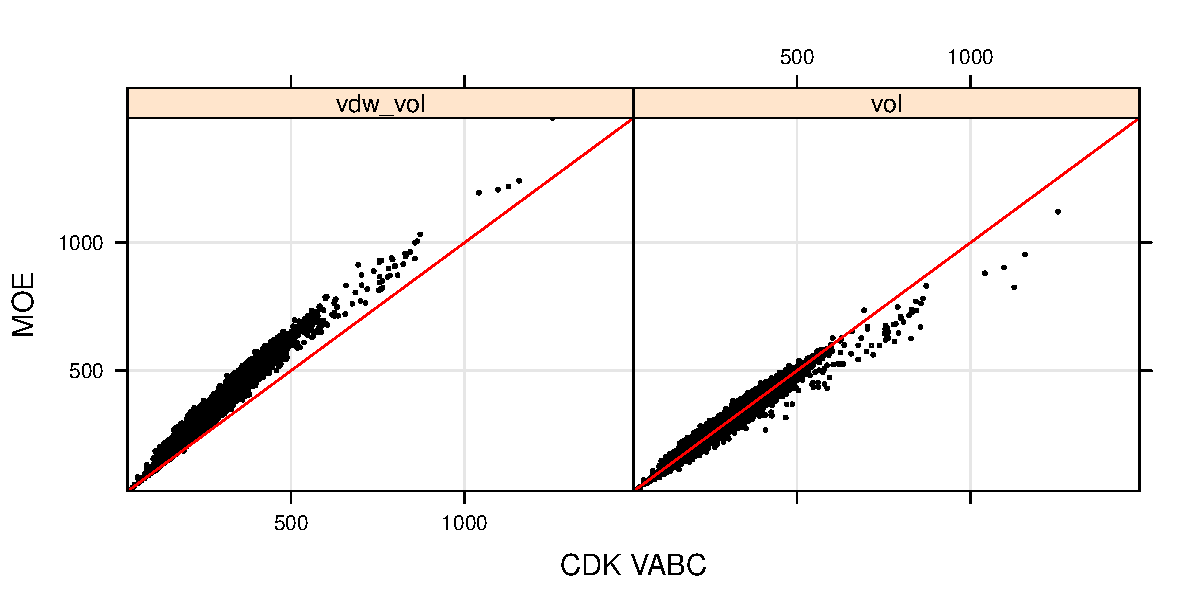
\includegraphics[width=\linewidth]{vol-moe-cdk}
}

\ctable[caption={Three tools to calculate descriptors: Bioclipse (top left), which allows selecting descriptor
implementations from various independent tools, CDK-Taverna (top right), which is an extension to Taverna
to calculate descriptors with the CDK, Ambit2 (bottom), which implements the OpenTox API providing
a REST-based API for descriptor calculation and wraps various descriptor calculation
tools.},cap={},label={fig:tools},botcap,figure]
{c}
{}
{
  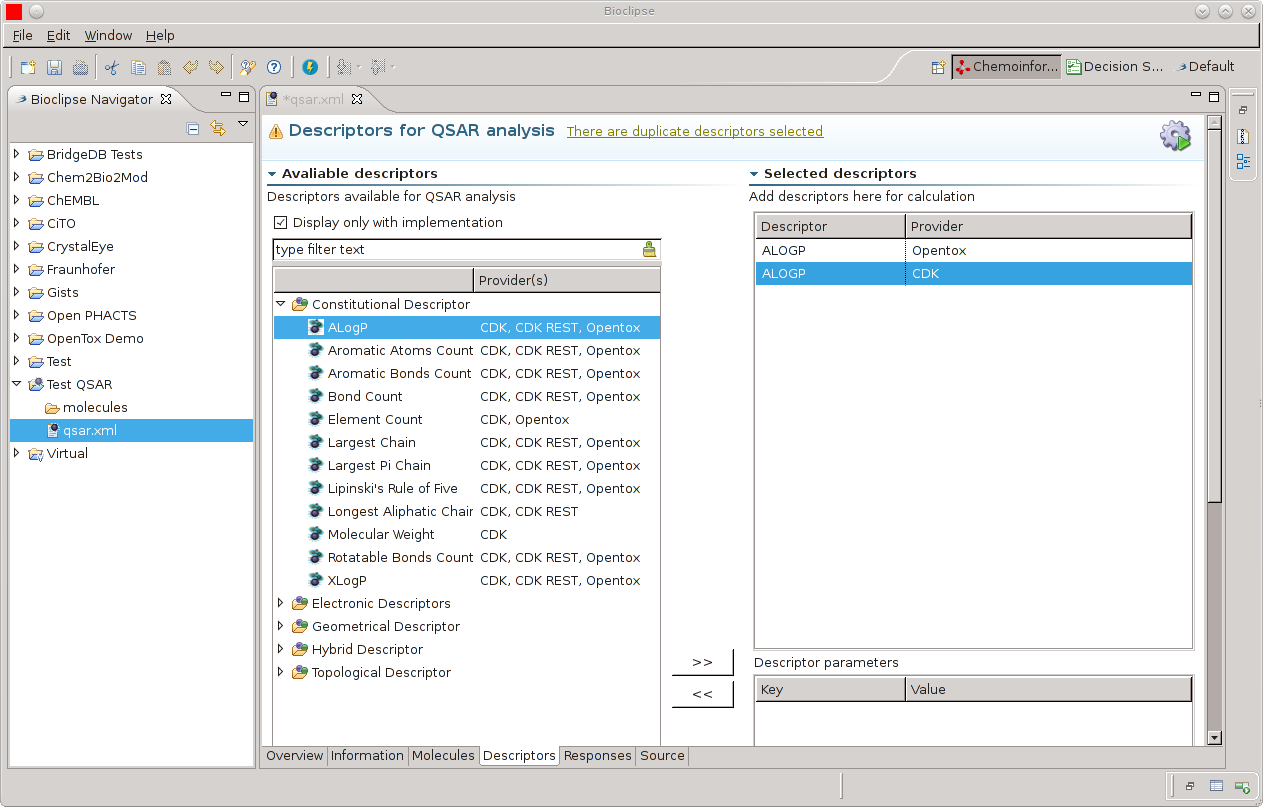
\includegraphics[width=0.48\linewidth]{bioclipse}
  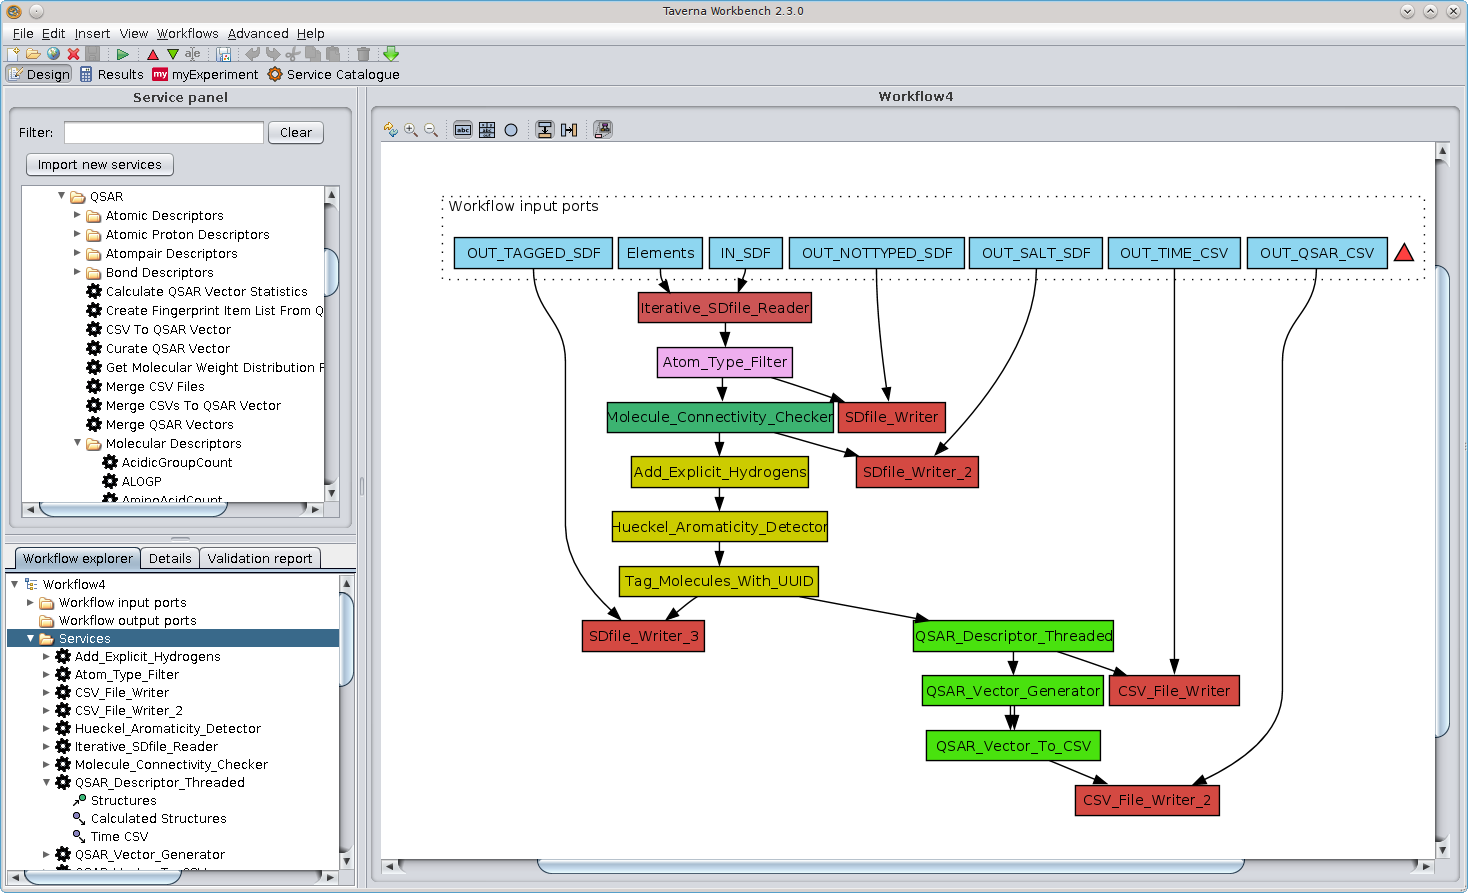
\includegraphics[width=0.48\linewidth]{cdktaverna} \\
  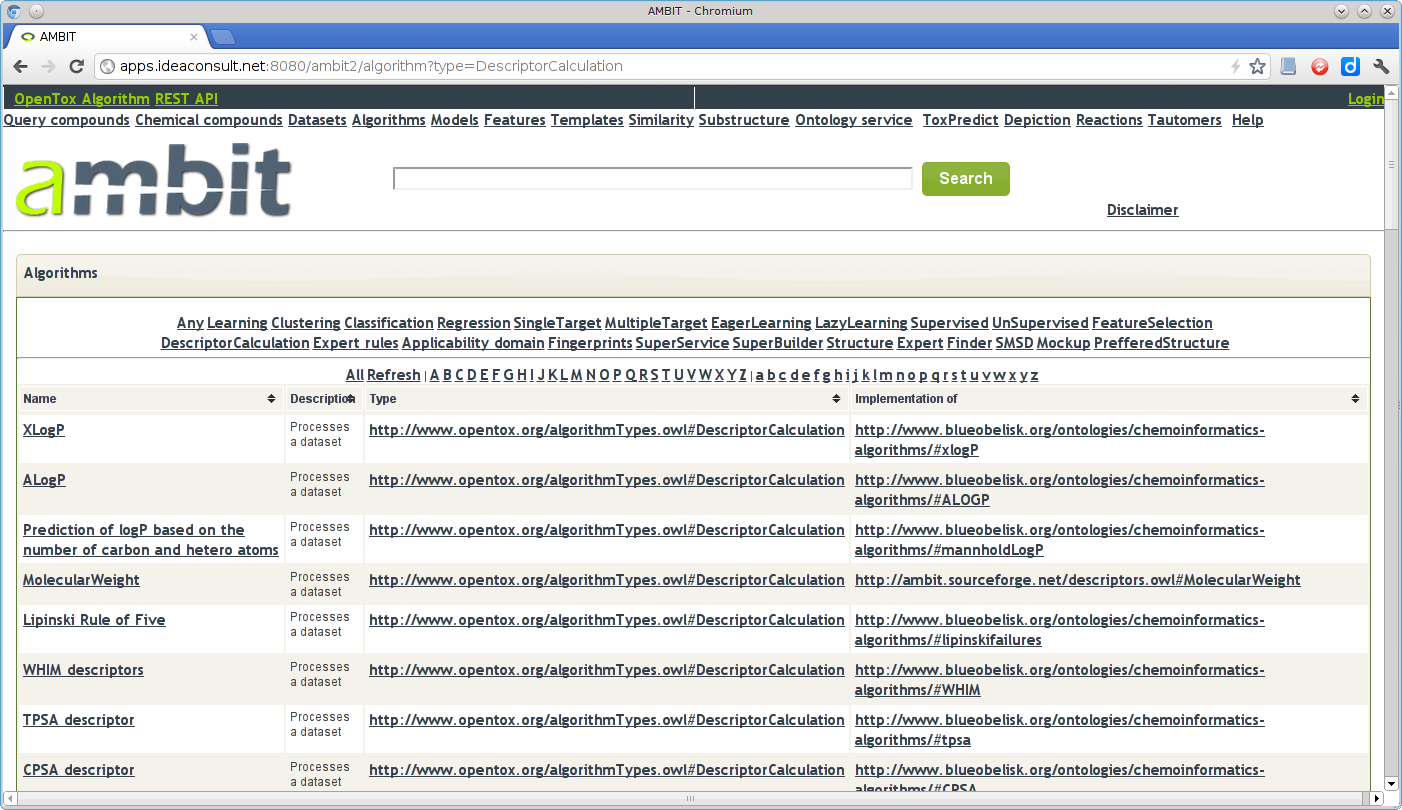
\includegraphics[width=0.48\linewidth]{ambitOnline}
}

\ctable[caption={UML diagram of the CDK descriptor API in version 1.4.},cap={},label={fig:cdkapi},botcap,figure]
{c}
{}
{
  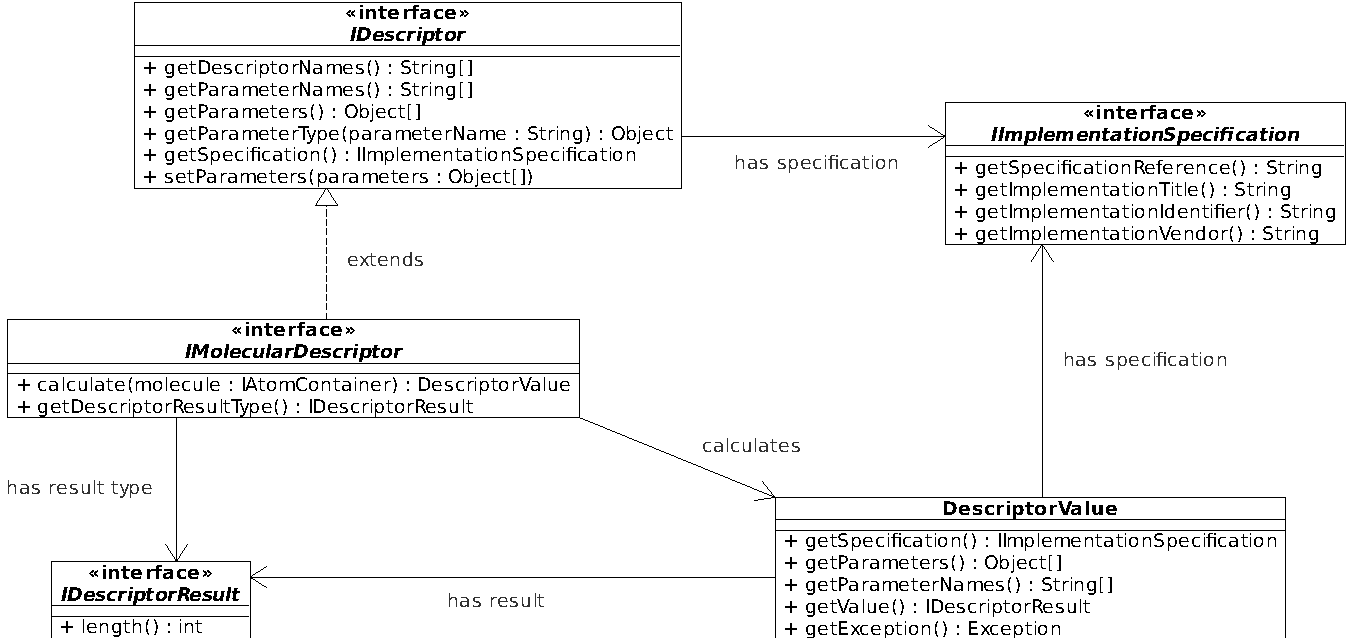
\includegraphics[width=\linewidth]{iDescriptor.pdf}
}

\ctable[caption={A comparison of Topological Polar Surface Area values
generated using the CDK and ACD Labs software, for 57,857 molecules
taken from Pubchem AID 1996.},cap={},label={fig:tpsa},botcap,figure]
{c}
{}
{
  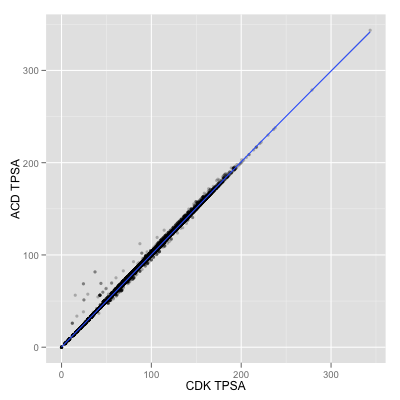
\includegraphics[width=\linewidth]{tpsa-cdk-acd}
}

\ctable[caption={A comparison of experimental versus calculated logP values
generated using the CDK, ACD Labs and ChemAxon software, for 10,000 molecules
taken from the proprietary logPstar dataset [REF?]},cap={},label={fig:logp},botcap,figure]
{c}
{}
{
  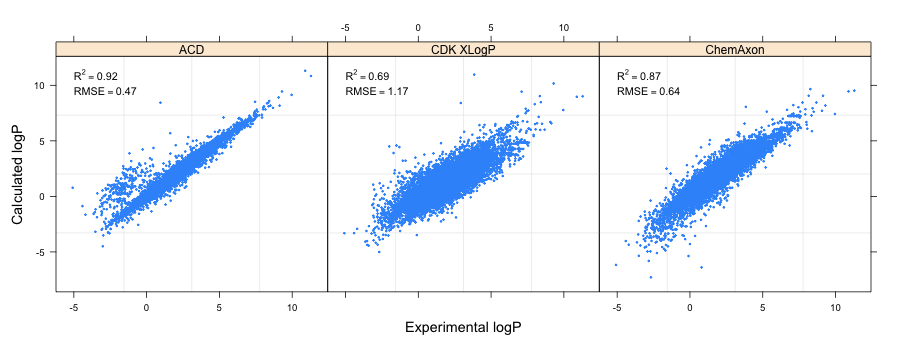
\includegraphics[width=\linewidth]{logp-comp-exptl}
}

\end{document}
  
    
     